\section{Introduction}

As code agents rapidly advance, evaluation evolves along two dimensions: from evaluating models that generate code in a single response to agents that sustain tool-driven interaction, and from function-level generation to repository-level workflows. HumanEval and MBPP represent the former setting, whereas SWE-bench evaluates repository-scale bug repair and Terminal-Bench covers command-line agent tasks~\cite{chen2021evaluating,austin2021program,jimenez2024swebench,merrill2026terminalbench}.

% \wslcomment{At a high level, program verification builds a machine-checkable chain from what a program should do to what its implementation actually does. This chain comprises three stages. \emph{Stage I: Contract} states the program's intended behavior via pre-/post-conditions. \emph{Stage II: Auxiliary Annotation} introduces logical assertions at intermediate control-flow points, notably loop invariants, which serve as the basis for generating  verification conditions in the subsequent stage. \emph{Stage III: Proof} generates verification conditions (VCs) through program reasoning and discharges them via automated or interactive theorem proving; a successful discharge formally certifies that the implementation satisfies its contract. These stages are tightly coupled: a proof failure often necessitates upstream revisions, e.g., modifying the contract, or strengthening a loop invariant, before re-verification.}

At a high level, program verification builds a machine-checkable chain from what a program should do to what its implementation actually does. This chain comprises three stages. \emph{Stage I: Contract} states the program's intended behavior through pre-/postconditions. \emph{Stage II: Auxiliary Annotation} adds facts needed at intermediate program points, such as loop invariants. A verification-condition generator (VCG) then automatically analyzes the implementation, contract, and auxiliary annotations to produce proof goals. \emph{Stage III: Proof} constructs machine-checkable proofs  for these goals, in our case, Rocq scripts. Once Rocq accepts all proofs, the implementation is formally shown to satisfy its contract. These stages are tightly coupled. A failed proof may require repairing the proof or revising the annotations, after which VCG is rerun and the new proof goals are checked again. While the contract may also be revised in the general case, our primary task fixes it and focuses on the annotation–proof interplay. We additionally provide an end-to-end task that requires generating the contract as well.

This iterative, feedback-driven process, where verification benefits greatly from holistic awareness of the surrounding verification context (e.g.,  inductive predicates and reusable proof lemmas), makes formal C verification particularly well suited to repository-level agent evaluation. It combines program-semantic reasoning and theorem proving, exercising both code and mathematical capabilities. A deterministic audit checks whether the agent succeeds and prevents cheating. 

%\wslcomment{Existing formal-verification benchmarks, however, expose only isolated fragments of this workflow. ATP-based suites focus on generating contracts or auxiliary annotations but delegate the proof discharge to  automated verifiers~\cite{lecong2025formalbench,loughridge2024dafnybench,sun2024clover}; ITP-based benchmarks start from pre-established contracts and annotations and focus solely on constructing proofs~\cite{thakur2025clever,ye2026verina,miranda2026veribench,dougherty2025proving,xu2026neural,xin2026verisoftbench}. Neither evaluates the agent's ability to handle the tight coupling between auxiliary annotations and proofs, including returning upstream when a failed proof exposes a missing intermediate fact.}

Existing formal-verification benchmarks, however, usually evaluate only part of this process. Some focus on generating contracts or auxiliary annotations and rely on automated verifiers to complete the proof~\cite{lecong2025formalbench,loughridge2024dafnybench,sun2024clover}. Other benchmarks focus on proof generation.  Whether the implementation and contract are provided or generated by the model, they are fixed before proof begins, and the model is evaluated only on constructing the proof~\cite{thakur2025clever,ye2026verina,miranda2026veribench,dougherty2025proving,xu2026neural,xin2026verisoftbench}. Neither paradigm evaluates whether a code agent can iteratively coordinate auxiliary annotations and proofs, including revising the auxiliary annotations when a failed proof reveals a missing fact.

C program verification is  particularly challenging because the language provides no native contract or proof layer and exposes low-level execution details. Contracts and auxiliary annotations must account for not only the intended functional behavior but also low-level properties, such as  pointer aliasing, mutable arrays and strings, memory ownership, integer overflow, and other forms of undefined behavior. The proof must connect these low-level facts back to the top-level contract. When a proof fails, the agent may need to repair the proof or strengthen the  annotations, making even short functions a long-horizon task.

We introduce \textsc{CAV-Bench}, to our knowledge the first benchmark of formally verified HumanEval implementations in C. It contains 140 human-reviewed and formally verified C programs with complete contract, annotations, and proof artifacts as ground-truth references. In its primary task, \textsc{CAV-Bench} gives an agent a repository containing the C implementation and contract to be verified, and asks the agent to complete the auxiliary annotation and proof stages within the repository. Unlike benchmarks that ask a model to synthesize a new program, \textsc{CAV-Bench} evaluates whether an agent can formally verify a given C implementation against its contract.

\begin{figure*}[t]
\centering
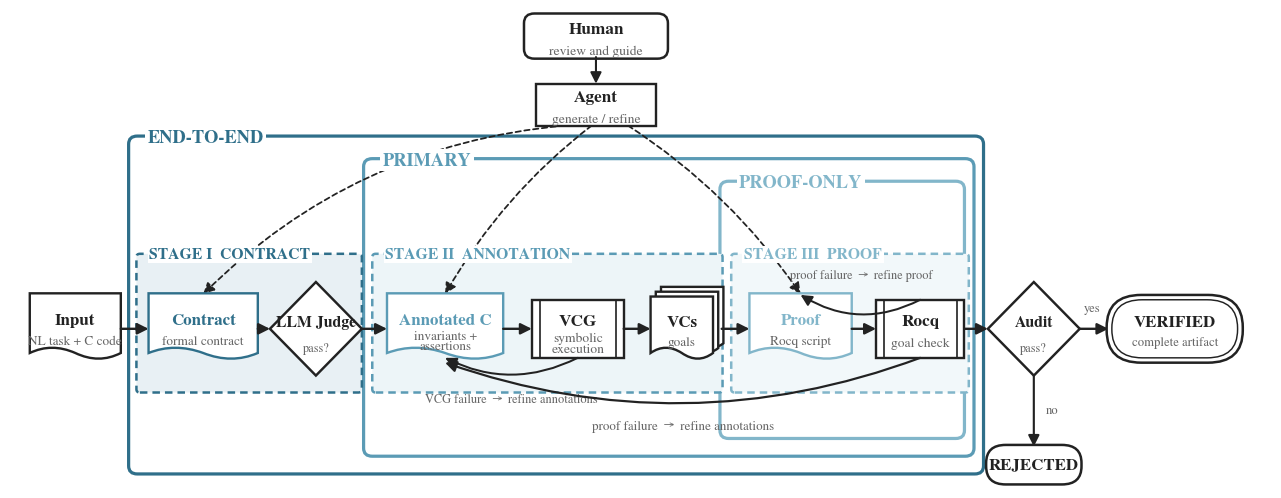
\includegraphics[width=0.94\textwidth]{figures/task_design_agentic.png}
\caption{The \textsc{CAV-Bench} construction and evaluation pipeline.}
\label{fig:task-design}
\end{figure*}

Figure~\ref{fig:task-design} summarizes the workflow. The primary task fixes the contract and evaluates the auxiliary annotation and proof stages. We additionally provide an end-to-end task that evaluates all three stages and a proof-only task that supplies the contract and auxiliary annotations to isolate the proof stage. Across all tasks, a deterministic audit checks the submitted artifacts and decides success rather than relying on the agent's own claim.

We conduct extensive experiments across frontier code-agent and model configurations and multiple reasoning-effort levels. Even the strongest evaluated configuration, Codex with GPT-5.5 at xhigh effort, verifies only 57.1\% of the 140 primary-task instances within the 90-minute budget. Accepted runs still require tens of minutes, millions of input tokens, and repeated repository and checker interaction. These results leave substantial room to improve not only verification accuracy, but also trajectory efficiency, stopping behavior, and time and token cost.

Our contributions are:
\begin{itemize}
    \item \textbf{A HumanEval benchmark for formal C verification:} 140 tasks pairing natural-language problem descriptions with executable C implementations (adapted from C++ as no C version existed) and their formal  contracts. Verification revealed discrepancies in several original solutions.
    \item \textbf{Human-in-the-loop construction of fully verified ground truth:} experts guide a code agent to produce complete auxiliary annotations and Rocq proofs, all checked by a deterministic audit.
    \item \textbf{Three agent tasks with experimental baselines:} contract-to-proof, end-to-end, and proof-only tasks, plus large-scale measurements of yield, reasoning effort, stage coupling, termination failures, and tool-use iteration.
\end{itemize}
